\section{Использование предложенных алгоритмов токенизации изображений для решения различных нейросетевых задач обработки изображений}

В этой главе рассматривается применение построенных токенизаторов для решения различных нейросетевых задач обработки изображений. Ранее, в предыдущей главе, уже была решена задача многоклассовой классификации изображений. В этой главе также решаются задача регрессии и задача генерации изображений.

\subsection{Решение задачи регрессии}

Решение задачи регрессии было выполнено с использованием набора данных UTKFace. Данный набор данных содержит 23 708 изображений лиц, а также соответсвующих данным изображениям аннотаций возраста (от 0 до 118 лет, распределение возрастов равномерное), пола и этноса. С помощью данного набора данных решалась задача определения возраста человека по изображению его лица. Исходная выборка была разделена на тренировочную с 18966 изображениями лиц и их аннотациями и валидационную с 4742 изображениями лиц с соответствующими аннотациями.

Все изображения считываются как трехканальные и масштабируются до размера 128, предобработка изображений, а также случайная аугментация совпадает с предобработкой и аугментацией во время решения задачи многоклассовой классификации.

В качестве модели трансформера использовалась модель с той же архитектурой, как и при решении задачи классификации. 

Для построения модели регрессора по токену класса выходной последовательности был использован многослойный перцептрон со следующей архитектурой:

\begin{itemize}
    \item Линейный полносвязный слой с количеством входов, равным размерности токенов трансформера, и со 128 выходами,
    \item Функция активации LeakyReLU,
    \item Линейный полносвязный слой с одним выходом.
\end{itemize}

Итоговая модель преобразует предобработанное изображение, используя следующую последовательность модулей:

\begin{itemize}
    \item Токенизатор изображений,
    \item Модель трансформер,
    \item Модель регрессор.
\end{itemize}

Для обучения задачи регрессии использовалась функция потерь, основанная на средней квадратичной ошибке:

$$
\mathcal{L}_{\mathrm{MSE}} = \frac{1}{N} \sum_{i=1}^{N} \bigl(y_i - \hat{y}_i\bigr)^2,
$$

где: 

\begin{itemize}
  \item $N$ — число объектов в выборке,
  \item $y_i$ — истинное значение целевой переменной для $i$-го объекта,
  \item $\hat{y}_i$ — предсказанное моделью значение целевой переменной для $i$-го объекта.
\end{itemize}

Для оценки качества обучения модели использовалась метрика средней абсолютной ошибки:

$$
\mathrm{MAE} = \frac{1}{N} \sum_{i=1}^{N} \bigl|y_i - \hat{y}_i\bigr|,
$$

Поскольку эта метрика оценивает ошибку предсказания модели, то идеальным результатом является достижение показателя 0 при использовании этой метрики. В свою очередь, чем больше значение этой метрики, тем выше значение ошибки.

\subsubsection{Решение задачи регрессии моделью с токенизатором, основанным на быстром преобразовании Фурье}

Задача регрессии была решена модель с токенизатором, основанным на быстром преобразовании Фурье. Результаты обучения представлены в \autoref{table:mfft-regression}:

\begin{table}[H]
  \centering
  \begin{tabular}{|l|c|c|}
    \hline
    Метод токенизации & MSE & MAE \\ \hline
    FFT-токенизация & 115.89 & 10.77 \\
    \hline
  \end{tabular}
  \caption{Результаты обучения модели с токенизатором, основанном на быстром преобразовании Фурье для решения задачи регрессии по изображению.}
  \label{table:mfft-regression}
\end{table}

Видно, что средняя абсолютная ошибка составляет примерно 11 лет. На такое высокое значение ошибки влияет то, что возраст старых людей тяжелее определить по внешнему виду. Однако, в случае, если бы модель не была бы работоспособной, средняя абсолютная ошибка была бы значительно больше.


\subsubsection{Решение задачи регрессии моделью с токенизатором mSVD}

Далее задача регрессии была решена модель с токенизатором mSVD. Результаты обучения представлены в \autoref{table:msvd-regression}:

\begin{table}[H]
  \centering
  \begin{tabular}{|l|c|c|}
    \hline
    Метод токенизации & MSE & MAE \\ \hline
    mSVD-токенизация & 86.33 & 9.30 \\
    \hline
  \end{tabular}
  \caption{Результаты обучения модели с токенизатором mSVD для решения задачи регрессии по изображению.}
  \label{table:msvd-regression}
\end{table}

Видно, что средняя абсолютная ошибка составляет чуть больше 9 лет. Результаты немного лучше, чем представленные в \autoref{table:mfft-regression}. Таким образом, токенизатор mSVD работоспособен для решения задачи регрессии.

\subsection{Генерация изображений с использованием предложенных методов токенизации}
Исследуется применение предложенных методов токенизации для генерации изображений. Сначала рассматривается генерация изображений методом автокодировщика с использованием токенизатора на основе быстрого преобразования Фурье и с использованием токенизатора mSVD. Далее рассматривается авторегрессионная генерация изображений моделью трансформер-декодеровщик с использованием mSVD. Авторегрессионная генерация с использованием токенизатора на основе быстрого преобразования Фурье не рассматривается, поскольку обратное преобразование Фурье не способно восстановить утеренную при использовании низкочастотного фильтра информацию.

Для генерации изображений методом автокодировщика необходимы модели кодировщика и декодировщика. В качестве кодировщика был использован токенизатор, а в качестве декодировщика - соответствующий ему дотокенизатор. Итого, подобная модель будет иметь следующую архитектуру:

\begin{enumerate}
    \item Модель токенизатор,
    \item Линейный слой, имеющий входную и выходную размерность, равную размерностям токенов, функция активации LeakyReLU и слой прореживания с вероятностью зануления выхода нейронов равной 0.5,
    \item Модель детокенизатор.
\end{enumerate}

Детокенизацией последовательности токенов в изображение будем называть операцию обратную токенизации.

\subsubsection{Использование алгоритма токенизации, основанного на быстром преобразовании Фурье}

Рассмотрим архитектуру детокенизатора на основе быстрого преобразования Фурье. Детокенизатор строится как отраженный токенизатор. В начале, набор векторов размерности

$$
\Big(\dfrac{M^2}{16^2}, s_E\Big)
$$

преобразуется в тензор размерности

$$
\Big(s_E, \dfrac{M}{16}, \dfrac{M}{16}\Big).
$$

Следом,  полученный тензор обрабатывается последовательностью алгоритмов пиксельных перемешиваний, функций активации и свёрточных слоёв c размером ядра свёртки 3, шагом 1, отступом 1 и с нейроном смещения. Всего, используется 4 блока:

\begin{enumerate}
    \item Свёрточный слой,
    \item Слой нормализации,
    \item Функция активации LeakyReLU,
    \item Слой пиксельного перемешивания
\end{enumerate}

После чего, полученный тензор проецируется с помощью свёрточного слоя проекции с размером ядра свёртки 1, шагом 1, отступом 0 и без нейрона смещения. Полученный тензор имеет форму

$$
(6, M, M).
$$

Над данным тензором выполняется обратное быстрое преобразование Фурье, в результате получается трёхканальное изображение. 

% Сюда картинку схемы бы

Результаты генерации обученной модели с токенизатором на основе быстрого преобразования Фурье представлены на \autoref{fig:mfft-gen}.

\begin{figure}[H]
    \centering
    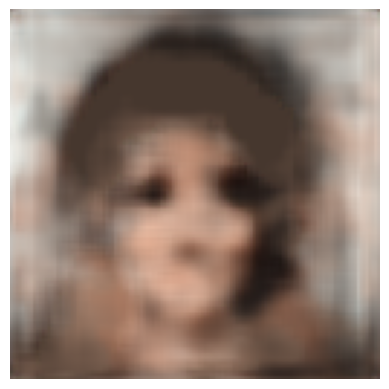
\includegraphics[width=0.5\textwidth]
    {images/generation/mfft_gen1.png}
    \caption{Пример генерации изображений с использованием токенизации на основе быстрого преобразования Фурье.}
    \label{fig:mfft-gen}
\end{figure}

Поскольку ''генерирующая'' модель, которая преобразовывает признаки очень слабая - всего один линейный полносвязный слой, то и результат генерации довольно слабый. Однако, детокенизатор все равно способен воссоздать изображение из набора векторов.

\subsubsection{Использование алгоритма токенизации mSVD}

Рассмотрим архитектуру детокенизатора mSVD. Детокенизатор mSVD строится как отраженная копия токенизатора mSVD. В начале, набор векторов размерности

$$
\Big(\dfrac{M^2}{16^2}, s_E\Big)
$$

преобразуется в тензор размерности

$$
\Big(s_E, \dfrac{M}{16}, \dfrac{M}{16}\Big)
$$

Следом, полученный тензор обрабатывается последовательностью алгоритмов пиксельных перемешиваний, функций активации и свёрточных слоёв c размером ядра свёртки 3, шагом 1, отступом 1 и с нейроном смещения. Однако, поскольку в mSVD токенизаторе присутстовало две ветви нейронных сетей, ответственных за получение наборов векторов $u$ и $v$ соответственно, то для поддержания симметрии токенизатора и детокенизатора, вместо одного свёрточного слоя на один этап пиксельного перемешивания, используется 2 свёрточных слоя.

Таким образом, детокенизатор mSVD имеет 4 блока. Каждый блок состоит из следующей последовательности слоев:

\begin{enumerate}
    \item Свёрточный слой,
    \item Слой нормализации,
    \item Функция активации LeakyReLU,
    \item Свёрточный слой,
    \item Слой нормализации,
    \item Функция активации LeakyReLU
    \item Слой пиксельного перемешивания
\end{enumerate}

Полученный после преобразования тензор имеет размерность 

$$
\Big(\dfrac{s_E}{16^2},  M, M\Big)
$$

Данный тензор проецируется в трехканальное изображение с помощью слоя проекции. Данный слой представлен в виде свёрточного слоя с размером ядра свёртки 1, шагом свёртки 1, размером отступа 0 и без нейрона смещения. 

% Сюда картинку схемы бы

Результаты генерации обученной модели на основе mSVD токенизатора на \autoref{fig:msvd-gen}.

\begin{figure}[H]
    \centering
    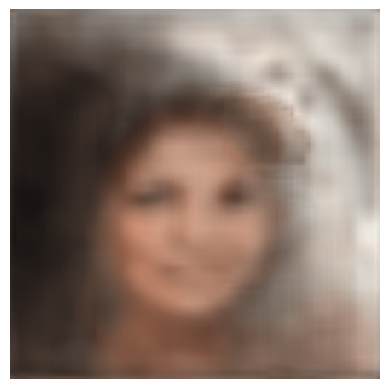
\includegraphics[width=0.5\textwidth]
    {images/generation/msvd_gen1.png}
    \caption{Пример генерации изображений с использованием mSVD токенизации.}
    \label{fig:msvd-gen}
\end{figure}

Проблемы генерации с использованием mSVD аналогичны проблемам генерации с использованием токенизатора на основе быстрого преобразования Фурье. 

\subsubsection{Авторегрессионная безусловная генерация изображений с использованием mSVD-токенизатора}

Для авторегрессионной безусловной генерации была построена модель трансформера декодировщика, аналогичная модели, предложенной в оригинальной работе \cite{transformer} без использования слоев перекрестного внимания (поскольку отсутствует какое-либо дополнительное условие).

Исходное изображение преобразуется в последовательность токенов с помощью предобученного токенизатора. После обработки последовательности токенов трансформером, результат декодируется в изображение с помощью предобученного детокенизатора.

Процесс обучения соответствует обучению процессу обучения из оригинальной статьи. В качестве функции потери была выбрана средняя квадратичная ошибка.

Генерация изображений происходит в авторегрессионном стиле: токен за токеном. Результат декодируется с помощью предобученного детокенизатора.


Результаты генерации обученной модели трансформера декодировщика с использованием mSVD токенизатора и mSVD детокенизатора представлены на \autoref{fig:autoregression-gen}

\begin{figure}[H]
    \centering
    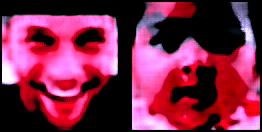
\includegraphics[width=0.75\textwidth]
    {images/generation/autoregression_gen.png}
    \caption{Пример генерации авторегрессионной генерации изображений с использованием токенизатора mSVD и детокенизатора mSVD.}
    \label{fig:autoregression-gen}
\end{figure}

Авторегрессионная генерация с использованием mSVD позволила достичь лучшего результата, чем генерация методом автокодировщика. Однако можно заметить, что при генерации изображения лучше всего были переданы низкочастные признаки, в то время как высокочастотные либо оказались утеряны, либо привели к ошибкам генерации.

Дальнейшее улучшение качества генерации заключается в изменении генеративной модели. К возможным способам улучшить качество генерируемых изображений относится квантизация токенов и добавление генеративно-состязательных нейронных сетей. Однако, данная тема лежит за пределами исследуемой в работе области.

\subsubsection{Выводы по главе 4}

В этой главе была исследована возможность обучения полученных в предыдущей главе токенизаторов для решения различных нейросетевых задач обработки изображений, а именно регрессии и генерации. В результате, модели токенизаторов показали свою работоспособность.   

